\newenvironment{mtrx}[1]
{\begin{tiny}
 \begin{center}
	\hspace{-40pt}
	\vspace{-10pt}
 \begin{tabular}{r|c|c|}
	\multicolumn{1}{c}{} & \multicolumn{1}{c}{aviso} & \multicolumn{1}{c}{pop} \\
	\cline{2-3}
	me & #1  & #1  \\
	\cline{2-3}
	chelton  & #1 & #1  \\
	\cline{2-3}
\end{tabular}
 \end{center}
\end{tiny}
}


\begin{spacing}{.5}

\begin{frame}
	\mtrx{U}
	\begin{figure}
	\centering
	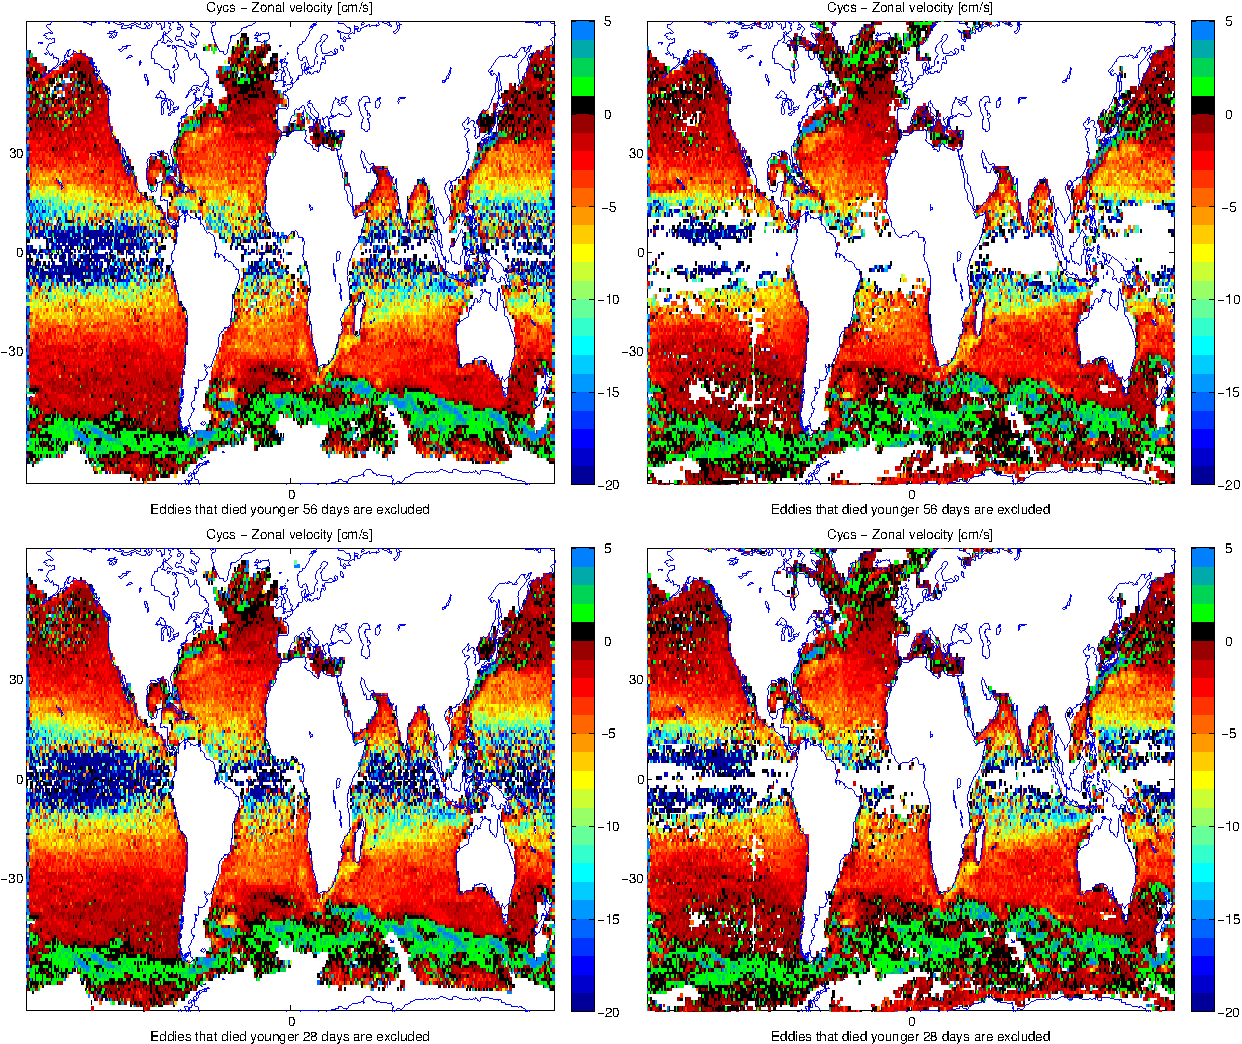
\includegraphics[height=220pt,keepaspectratio=true]{MUall.pdf}
	\end{figure}
\end{frame}

\begin{frame}
	\mtrx{zonal mean U}
	\begin{figure}
		\centering
		%\vspace{-10pt}
		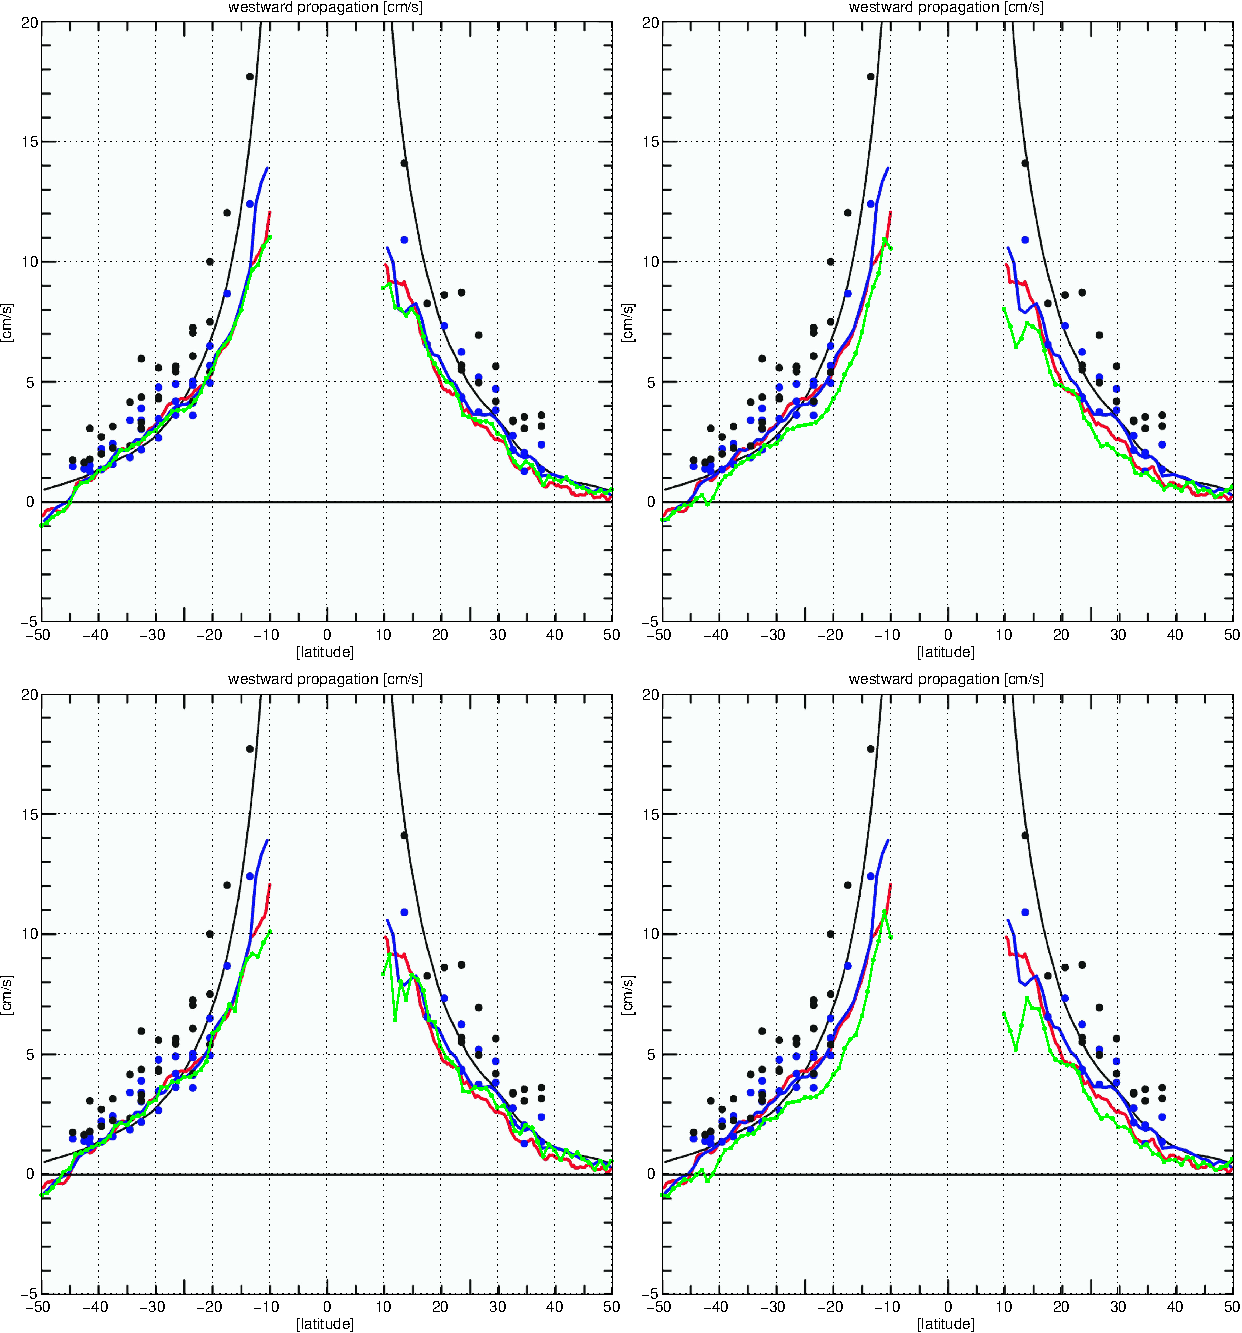
\includegraphics[height=210pt,keepaspectratio=true]{ZUall.pdf}
		\vspace{-10pt}
		\caption{
			\begin{tiny}
				 black dots: Radon transforms of 20°x10° high-pass filtered SSH fields along the 45 zonal sections. Red dots: means of $U$ along those sections (age $\ge 16$ weeks). red line: zonalmean(U). blue line: space-time-lagged cross-correlation (Fu 2009).
			\end{tiny}
		}
	\end{figure}
\end{frame}


\begin{frame}
\mtrx{$\sigma$}
 \begin{figure}
\centering
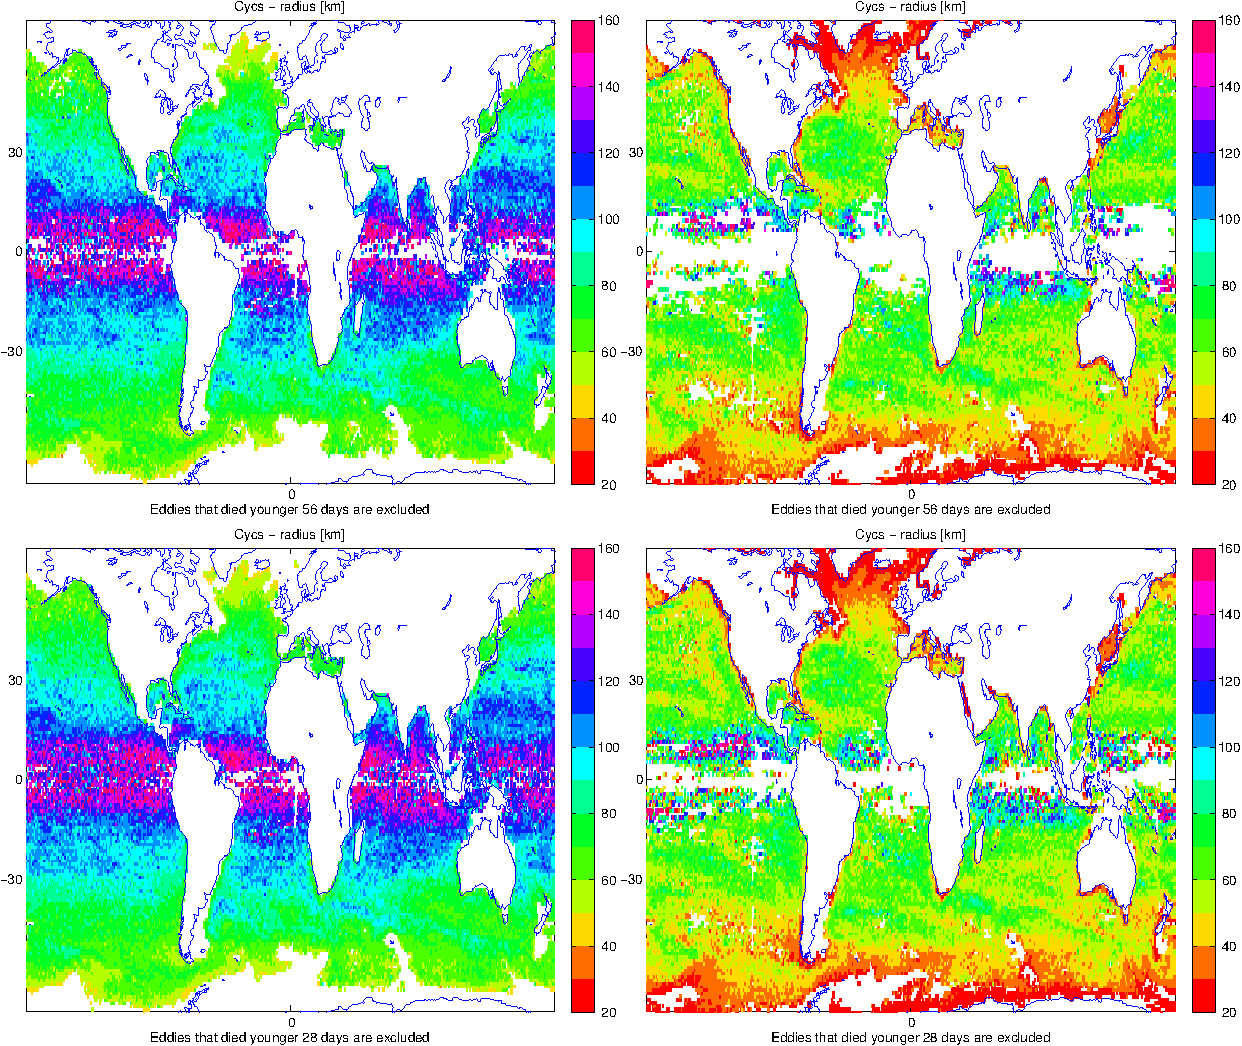
\includegraphics[height=220pt,keepaspectratio=true]{MRall.pdf}
\end{figure}
\end{frame}

\begin{frame}
\mtrx{zonal mean $\sigma$}
\begin{figure}
\centering
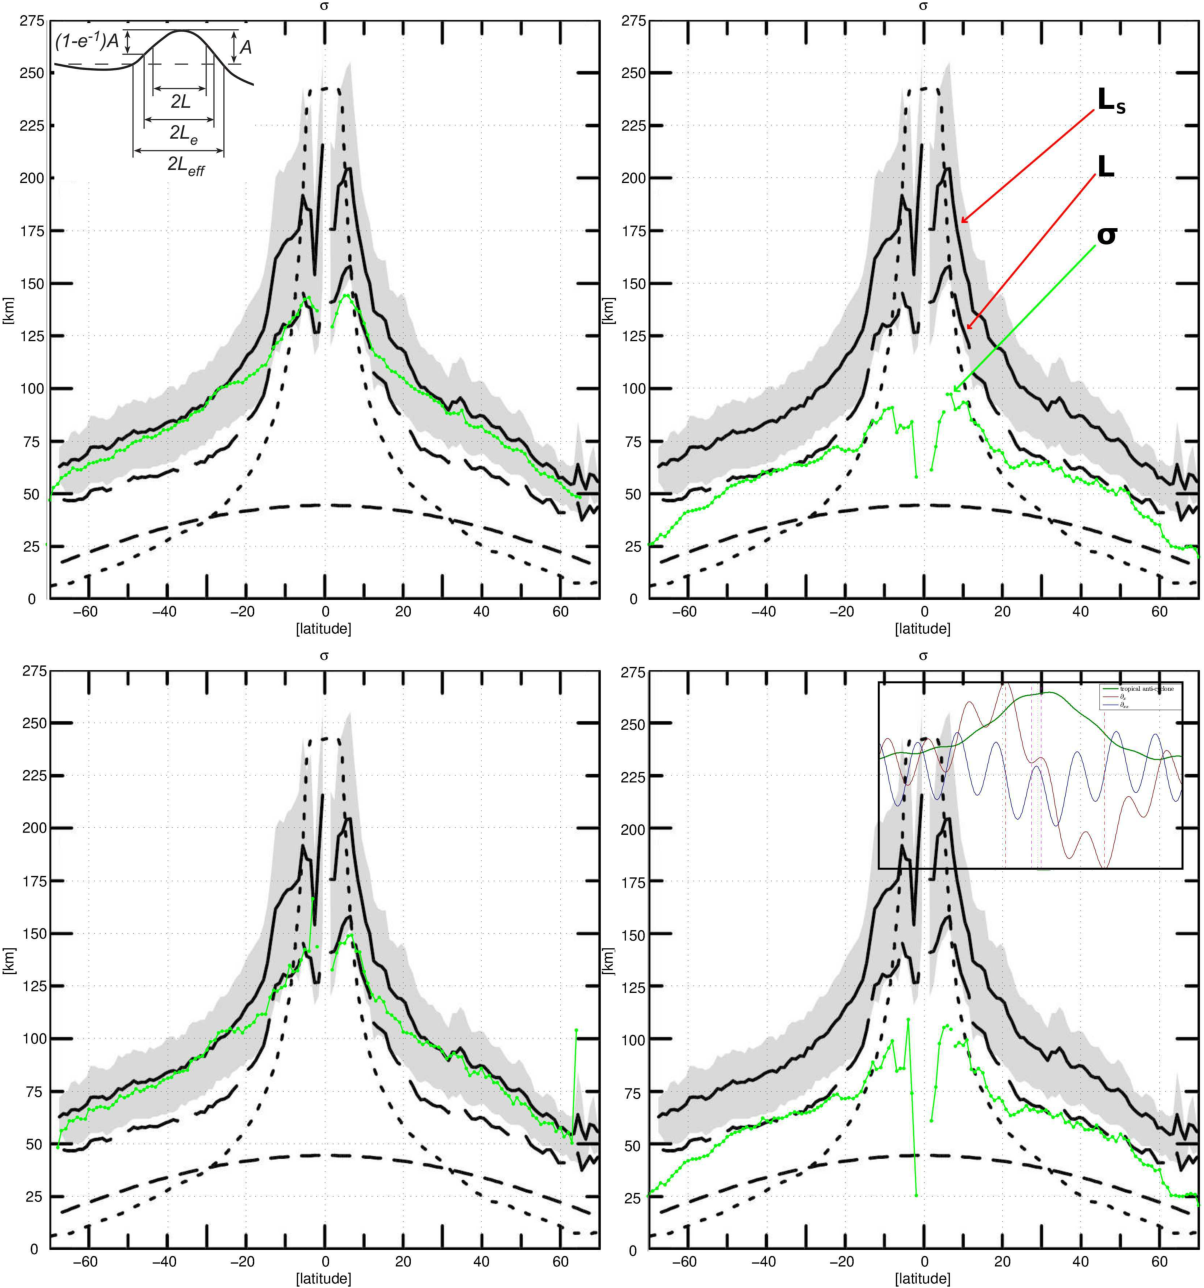
\includegraphics[height=220pt,keepaspectratio=true]{ZRall_anot.pdf}
\end{figure}
\end{frame}



\end{spacing}
